% Chapter Template

\chapter{All about classification} % Main chapter title

\label{Chapter6} % Change X to a consecutive number; for referencing this chapter elsewhere, use \ref{ChapterX}

\lhead{Chapter 6. \emph{All about classification}} % Change X to a consecutive number; this is for the header on each page - perhaps a shortened title

\section{Ensemble Methods}

A single phrase to describe ensemble methods is \textbf{Collective Intelligence}. A single source of information or suggestion is seldom a good idea. Using multiple sources of information and then using reduction methods on the outputs to reach the decision is better (well, most of the time). So there are \textbf{workers}, which are trained to do the heavy lifting, and there is a \textbf{collector} which analyses the potential of each worker and gains collective intelligence. In boosting, it also uses the knowledge gathered so far into the next worker it builds. Ensemble method uses this technique and performs better in most of the cases than simple models like Linear Regression, Support Vector Machines, Nearest Neighbours, etc. Some simple ensemble techniques are \textbf{Max Voting}, \textbf{Averaging} and \textbf{Weighted Averaging}. Some more advanced techniques are \textbf{Stacking}, \textbf{Blending}, \textbf{Bagging} and \textbf{Boosting}. In both bagging and boosting, a sample of the dataset is selected with replacement and used as the data-"subset" for each worker's model.

\subsection{Bagging}

\begin{figure}[H]
\centering
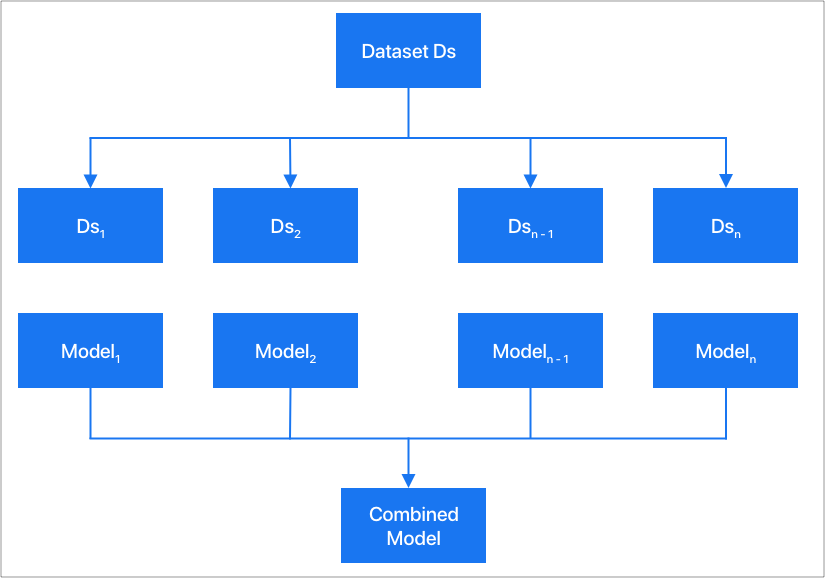
\includegraphics[height=7cm]{bagging.png}
\caption{Bagging}
\label{fig-6-1}
\end{figure}

In bagging technique:
\begin{enumerate}
    \item Let the complete dataset be $D$. A random sampling is done on $D_s$ obtaining dataset $D_i$.
    \item $D_i$ is used as the dataset for the model $M_i$. Hence if there are $N$ bags, there will be $M_0, M_1, \ldots M_{n - 1}$ models.
    \item Each of the models are trained independently of each other (and hence, they can be trained in parallel). 
    \item The output of the ensemble model is reduced from the outputs of the underlying models. A common mode of reduction is voting for classification task and median for regression task.
\end{enumerate}

\subsection{Boosting}

\begin{figure}[H]
\centering
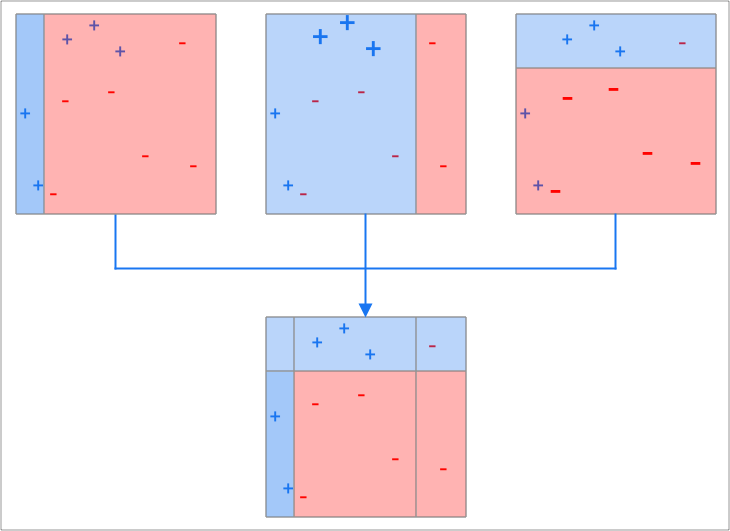
\includegraphics[height=7cm]{boosting.png}
\caption{Boosting}
\label{fig-6-2}
\end{figure}

In boosting technique:
\begin{enumerate}
    \item Let the complete dataset be $D$. A random sampling is done on $D$ obtaining dataset $D_i$.
    \item $D_i$ is used as the dataset for the model $M_i$.
    \item So, $M_i$ is trained first, and then the performance of the model is gauged on the complete dataset $D$.
    \item The mistakes or misclassification performed by the model is given more weightage. So the next model is biased against making the same mistake. So, the next model might make some other mistake, and then the one cretaed after it is biased against the new mistakes.
    \item This process is repeated $N$ number of times, creating $M_0, M_1, \ldots M_{n - 1}$.
    \item The output of the ensemble model is reduced from the outputs of the underlying models. A common mode of reduction is voting for classification task and median for regression task.
\end{enumerate}

\section{Models Used}
The ensemble models used in the experiment are XGBoost and Random Forest Classifier.

\subsection{Random Forest}

Random Forest is a bagging technique. It uses Decision Trees as the underlying worker models.

\subsection{XGBoost}

XGBoost is a boosting technique. It also uses Decision Trees as the worker models. The trees in XGBoost are not grown to full depth. Instead, the trees have fewer splits. A decision tree with a small depth is highly interpretable. A large number of trees, called estimators, often leads to overfitting. Hence, an early stooping criteria is often required to prevent it.

% Described below are the models used and their hyperparameters. Both of them are ensemble methods.

% \subsection{XGBoost}
